\section{Comparison and Discussion}
\label{sec:comparison-discussion}

The previous four sections reviewed the main technical routes from category-name-driven open-vocabulary segmentation to promptable masks, grounded language-mask alignment, reasoning segmentation, and extended video, 3D, remote-sensing, medical, and embodied scenarios. This section compares these routes along capability axes rather than by a single leaderboard. The central question is not only which method reports the highest number on a given benchmark, but what kind of openness, spatial precision, reasoning behavior, cost, and reproducibility that number actually supports.

Following the writing logic of the survey, Tables~\ref{tab:family-comparison}--\ref{tab:extended-comparison-evidence} serve different functions. Table~\ref{tab:family-comparison} is a method-family map. Tables~\ref{tab:representative-comparison-evidence} and~\ref{tab:extended-comparison-evidence} collect representative numerical or protocol facts from the original papers. These values should not be read as a unified ranking, because the benchmarks, metrics, backbones, training data, prompt protocols, and output formats differ substantially across tasks. They instead show why fair comparison requires reporting both the result and the setting that produced it.

\begin{table*}[t]
\centering
\small
\setlength{\tabcolsep}{4pt}
\renewcommand{\arraystretch}{1.32}
\caption{Comparison of major method families. The table records the interface and the main reporting condition required for fair comparison.}
\label{tab:family-comparison}
\begin{tabularx}{\textwidth}{>{\raggedright\arraybackslash}p{0.17\textwidth}>{\raggedright\arraybackslash}p{0.25\textwidth}>{\raggedright\arraybackslash}p{0.28\textwidth}>{\raggedright\arraybackslash}X}
\toprule
Method family & Main interface & Representative evidence anchor & Required comparison control \\
\midrule
CLIP-based dense alignment & Category names or text prompts are compared with patch, pixel, or cost-volume features & PnP-OVSS~\citep{luo2024pnpovss}, DPSeg~\citep{zzhaoDPSegDualpromptCost2025}, ITACLIP~\citep{maaydinItaclipBoostingTrainingfree2025}, CLIPer~\citep{lsunCliperHierarchicallyImproving2025}, CorrCLIP~\citep{dzhangCorrclipReconstructingPatch2025}, and Trident~\citep{shiyHarnessingVisionFoundation2025} repair CLIP spatial features with attention rewriting, DINO, SAM, or diffusion priors & Control input resolution, prompt templates, post-processing, and auxiliary foundation modules \\
Proposal-then-classification and segment embeddings & Class-agnostic masks or segments are classified by text-aligned region embeddings & OVSeg~\citep{liang2023ovseg}, SAN~\citep{xu2023san}, Mask-Adapter~\citep{yliMaskadapterDevilMasks2025}, USE~\citep{xwangUseUniversalSegment2024}, and ReME~\citep{xxuanReMEDataCentricFramework2025} improve masked-region recognition, CLIP-aware proposals, or segment-text reference data & Report mask generator, proposal budget, classifier backbone, and mask-text calibration \\
SAM and Grounded-SAM composition & Text, boxes, points, masks, detector outputs, or MLLM prompts drive SAM/SAM2 masks & SAM~\citep{kirillov2023sam}/SAM2~\citep{ravi2024sam2} supply mask priors, while Grounding DINO~\citep{liu2024groundingdino}, TGS-Agent~\citep{zhouThinkYouSegment2026}, AL-Ref-SAM2~\citep{huangUnleashingTemporalspatialReasoning2025}, and OpenWorldSAM~\citep{sgxiaoOpenworldsamExtendingSam22026} supply language grounding & Report prompt source, candidate count, grounding module, frame selection, and SAM/SAM2 variant \\
Region-word and pixel-grounded interfaces & Expressions, generated words, region features, masks, or location tokens are aligned with pixels & OneRef~\citep{xiaoOnerefUnifiedOnetower2024}, Mask Grounding~\citep{chngMaskGroundingReferring2024}, PixelLM~\citep{renPixellmPixelReasoning2024}, Osprey~\citep{yuanOspreyPixelUnderstanding2024}, GLaMM~\citep{rasheedGlammPixelGrounding2024}, and GroundingSuite~\citep{huGroundingSuiteMeasuringComplex2025} make language units spatially accountable & Evaluate response correctness, grounding correctness, and mask quality jointly \\
MLLM reasoning-to-mask generation & An MLLM infers targets and emits segmentation tokens, codebook tokens, proposals, boxes, or mask prompts & LISA~\citep{xlaiLisaReasoningSegmentation2024}, LLM-Seg~\citep{jwangLlmsegBridgingImage2024}, GSVA~\citep{xiaGsvaGeneralizedSegmentation2024}, PixelLM~\citep{renPixellmPixelReasoning2024}, OMG-LLaVA~\citep{zhangOmgllavaBridgingImagelevel2024}, LENS~\citep{zhuLensLearningSegment2026}, RISE~\citep{zhouReasoningImplicitSelfsupervised2026}, and SAM-R1~\citep{huangSamr1LeveragingSam2026} connect language reasoning to mask generation or reward optimization & Report faithfulness, rejection accuracy, token budget, decoder type, and reward design \\
Extended-domain reasoning and grounding & Video, audio, 3D, remote-sensing, medical, affordance, or embodied cues define the target & VideoLISA~\citep{baiOneTokenSeg2024}, ViLLa~\citep{zhengVillaVideoReasoning2025}, OVRSISBench~\citep{libExploringEfficientOpenvocabulary2026}, 3D-DRES~\citep{chen3DDRESDetailed3D2026}, Surprise3D~\citep{huangSurprise3dDatasetSpatial2026}, MedReasoner~\citep{yanMedreasonerReinforcementLearning2026}, and Affordance-R1~\citep{wangAffordancer1ReinforcementLearning2026} test temporal, geometric, domain, clinical, and functional constraints & Use domain-specific metrics; do not collapse temporal propagation, 3D grounding, clinical inference, or affordance localization into ordinary mIoU \\
\bottomrule
\end{tabularx}
\end{table*}

\begin{table*}[t]
\centering
\footnotesize
\setlength{\tabcolsep}{3pt}
\renewcommand{\arraystretch}{1.14}
\caption{Representative quantitative and protocol evidence from original papers. The rows are not directly comparable across tasks; they are included to show the settings behind common comparison claims.}
\label{tab:representative-comparison-evidence}
\begin{tabularx}{\textwidth}{>{\raggedright\arraybackslash}p{0.18\textwidth}>{\raggedright\arraybackslash}p{0.29\textwidth}>{\raggedright\arraybackslash}p{0.23\textwidth}>{\raggedright\arraybackslash}X}
\toprule
Evidence case and representative method & Verified setting from the paper & Reported result or protocol fact & What the result supports \\
\midrule
Masked-region recognition bottleneck: OVSeg~\citep{liang2023ovseg} & COCO-Stuff~\citep{caesar2018cocostuff}/COCO Captions~\citep{chen2015microsoft} training; zero-shot evaluation on ADE20K~\citep{zhou2017scene}, Pascal Context~\citep{mottaghi2014role}, and PASCAL VOC~\citep{everingham2015pascal} & With ground-truth masks but ordinary CLIP classification, ADE20K-150~\citep{zhou2017scene} reaches only 20.1 mIoU; with ordinary proposals but oracle classification, it reaches 66.5 mIoU. OVSeg-Swin-B~\citep{liang2023ovseg} reports 9.0/12.4/29.6/55.7/94.5 mIoU on A-847/PC-459/A-150/PC-59/PAS-20. & Mask quality and mask classification are separate bottlenecks; open-vocabulary gains cannot be attributed to masks alone \\
Lightweight CLIP-aware adaptation: SAN~\citep{xu2023san} & COCO-Stuff~\citep{caesar2018cocostuff} training; CLIP ViT-L/14~\citep{radford2021learning}; evaluation on ADE-847~\citep{zhou2017scene}, PC-459~\citep{mottaghi2014role}, ADE-150~\citep{zhou2017scene}, PC-59~\citep{mottaghi2014role}, and VOC~\citep{everingham2015pascal} & SAN~\citep{xu2023san} reports 12.4/15.7/32.1/57.7/94.6 mIoU on these five datasets, with 8.4M trainable parameters in the side adapter setting. & Parameter-efficient adaptation can improve dense recognition while keeping CLIP largely fixed, but comparisons must control backbone and ensemble choices \\
Training-free open-vocabulary segmentation: Trident~\citep{shiyHarnessingVisionFoundation2025} & Training-free composition of CLIP~\citep{radford2021learning}, DINO~\citep{caron2021emerging}, and SAM~\citep{kirillov2023sam}; eight benchmarks including VOC~\citep{everingham2015pascal}, Context~\citep{mottaghi2014role}, Object/Stuff from COCO-style datasets~\citep{lin2014microsoft,caesar2018cocostuff}, Cityscapes~\citep{cordts2016cityscapes}, and ADE~\citep{zhou2017scene} & With ViT-B/16, Trident~\citep{shiyHarnessingVisionFoundation2025} reports 67.1 VOC21, 38.6 Context60, 41.1 COCO Object, 84.5 VOC20, 42.2 Context59, 28.3 Stuff, 42.9 City, 21.9 ADE, and 45.8 average mIoU. & Training-free does not mean single-model or low-cost; auxiliary foundation modules and refinement prompts are part of the comparison \\
Hierarchical CLIP spatial repair: CLIPer~\citep{lsunCliperHierarchicallyImproving2025} & Training-free CLIP~\citep{radford2021learning} spatial repair with early-layer fusion and Stable Diffusion compensation~\citep{rombach2022high}; eight segmentation datasets & With ViT-B/16, CLIPer~\citep{lsunCliperHierarchicallyImproving2025} reports 66.5 VOC, 38.3 Context, 40.0 Object, 86.0 VOC20, 42.4 Context59, 28.6 Stuff, 38.7 Cityscapes, 22.0 ADE, and 45.3 average mIoU. & Improving spatial representation can raise open-vocabulary segmentation without pixel-label training, but diffusion-based compensation adds another reproducibility variable \\
Image reasoning segmentation: LISA~\citep{xlaiLisaReasoningSegmentation2024} & ReasonSeg~\citep{xlaiLisaReasoningSegmentation2024} with 239 training samples, 200 validation samples, and 779 test samples; gIoU/cIoU metrics & LISA-13B-LLaVA1.5~\citep{xlaiLisaReasoningSegmentation2024} with fine-tuning reports 65.0/72.9 gIoU/cIoU on ReasonSeg validation and 61.3/62.2 on the overall test set. & A small amount of reasoning segmentation data can substantially improve implicit-query segmentation, but the metric still mixes target inference and mask quality \\
Multi-target pixel reasoning: PixelLM~\citep{renPixellmPixelReasoning2024} & MUSE~\citep{renPixellmPixelReasoning2024} multi-target reasoning segmentation; no external SAM~\citep{kirillov2023sam} in PixelLM rows; compute reported in tera floating-point operations (TFLOPs) with gIoU/cIoU & PixelLM-Llama2-13B~\citep{renPixellmPixelReasoning2024} reports 42.3/51.0 test gIoU/cIoU on MUSE with 6.65 TFLOPs, while PixelLM-7B reports 39.2/46.3 with 3.57 TFLOPs. & More expressive mask tokenization and pixel decoding can improve multi-target reasoning while reducing dependence on external segmenters \\
\bottomrule
\end{tabularx}
\end{table*}

\begin{table*}[t]
\centering
\small
\setlength{\tabcolsep}{4pt}
\renewcommand{\arraystretch}{1.24}
\caption{Representative quantitative and protocol evidence for extended scenarios. These rows use task-specific metrics and should not be compared as a single leaderboard.}
\label{tab:extended-comparison-evidence}
\begin{tabularx}{\textwidth}{>{\raggedright\arraybackslash}p{0.18\textwidth}>{\raggedright\arraybackslash}p{0.29\textwidth}>{\raggedright\arraybackslash}p{0.23\textwidth}>{\raggedright\arraybackslash}X}
\toprule
Evidence case and representative method & Verified setting from the paper & Reported result or protocol fact & What the result supports \\
\midrule
Video reasoning segmentation: ViLLa~\citep{zhengVillaVideoReasoning2025} & VideoReasonSeg~\citep{zhengVillaVideoReasoning2025} contains 3k videos and 15k object-instruction pairs; metrics include segmentation $\mathcal{J}\&\mathcal{F}$ and multiple-choice accuracy & ViLLa-InternVideo2-6B~\citep{zhengVillaVideoReasoning2025} reports 55.4 overall $\mathcal{J}\&\mathcal{F}$ and 49.9 multiple-choice accuracy on VideoReasonSeg; it also reports 67.5/74.3/49.4 $\mathcal{J}\&\mathcal{F}$ on Ref-YouTube-VOS, Ref-DAVIS17, and MeViS under the same paper's protocol~\citep{zhengVillaVideoReasoning2025}. & Video methods must separate temporal mask propagation from video-language reasoning and answer accuracy \\
Remote-sensing open vocabulary: RSKT-Seg~\citep{libExploringEfficientOpenvocabulary2026} & OVRSISBench~\citep{libExploringEfficientOpenvocabulary2026} reformulates eight remote-sensing datasets and evaluates with mIoU and mACC under cross-dataset protocols & RSKT-Seg with ViT-L~\citep{libExploringEfficientOpenvocabulary2026} reports 36.76 m-mIoU and 57.91 m-mACC across the eight OVRSIS datasets; the paper also reports 65.11 ms mean inference time and 15.36 FPS for RSKT-Seg. & Domain-specific scale, rotation, and sensor priors change what open-vocabulary segmentation means in practice \\
Clinical reasoning grounding: MedReasoner~\citep{yanMedreasonerReinforcementLearning2026} & U-MRG-14K~\citep{yanMedreasonerReinforcementLearning2026} contains 14K image-mask pairs with implicit clinical queries and reasoning traces across 10 modalities, 15 super-categories, and 108 categories & MedReasoner-7B~\citep{yanMedreasonerReinforcementLearning2026} reports 32.42 IoU, 26.55 pDice, and 37.78 Dice on the U-MRG-14K test set with MedSAM2 fixed as the segmentation module. & Clinical grounding requires target interpretation and spatial prompting before segmentation; mask Dice alone does not reveal whether the clinical reasoning was correct \\
Affordance reasoning: Affordance-R1~\citep{wangAffordancer1ReinforcementLearning2026} & ReasonAff~\citep{wangAffordancer1ReinforcementLearning2026} in-domain evaluation plus zero-shot UMD and AGD20K evaluation under the Affordance-R1 protocol~\citep{wangAffordancer1ReinforcementLearning2026}; metrics are gIoU, cIoU, P50-95, and P50 & Affordance-R1~\citep{wangAffordancer1ReinforcementLearning2026} reports 67.41/62.72/74.50/55.22 on ReasonAff, 49.85/42.24/34.08/53.35 on UMD, and 31.78/27.85/7.99/20.49 on AGD20K. & Functional-region grounding should not be judged by object masks; action affordance and part-level reasoning need dedicated metrics \\
\bottomrule
\end{tabularx}
\end{table*}

\subsection{Comparison across method families}

Several conclusions can be drawn from Table~\ref{tab:family-comparison}. First, the literature is organized by interfaces as much as by architectures. Open-vocabulary segmentation uses category names or descriptions as the interface. Promptable segmentation uses points, boxes, masks, or detector outputs. Grounded segmentation uses expressions, regions, generated words, or conversations. Reasoning segmentation uses implicit instructions, rationales, rejection decisions, or reward-optimized traces. A method should therefore be compared with systems that receive a similar type of input and are expected to produce a similar type of output.

Second, spatial precision and semantic flexibility are usually supplied by different components. CLIP-style models provide open semantic recognition but weak local structure; SAM-style models provide strong masks but weak category semantics; MLLMs provide flexible instruction following but need a reliable bridge to pixels~\citep{radford2021learning,kirillov2023sam,xlaiLisaReasoningSegmentation2024}. Most strong systems are therefore hybrids. OVSeg adapts CLIP for masked regions, SAN makes mask proposals CLIP-aware, Trident composes CLIP, DINO, and SAM, Grounded-SAM pipelines combine grounding models with SAM, and reasoning systems connect LLM hidden states, segmentation tokens, proposals, or pixel decoders to masks~\citep{liang2023ovseg,xu2023san,shiyHarnessingVisionFoundation2025,liu2024groundingdino,renPixellmPixelReasoning2024}. This makes component disclosure as important as final accuracy.

Third, the harder the language interface becomes, the less sufficient a single mask metric becomes. mIoU is appropriate for category-level dense classification. IoU, cIoU, or gIoU better match referring or reasoning masks. $\mathcal{J}\&\mathcal{F}$ is needed for video masks. Grounded conversation needs response-mask consistency, false-premise handling, and hallucination checks. Medical and affordance grounding need target interpretation and domain-specific correctness~\citep{wuSeeSaySegment2024,guoSeeingBelievingRichContext2026,yanMedreasonerReinforcementLearning2026,wangAffordancer1ReinforcementLearning2026}. Thus, a comparison section should explain which capability each metric can and cannot prove.

\subsection{Semantic openness versus spatial precision}

The core trade-off in open-vocabulary and reasoning segmentation is semantic openness versus spatial precision. CLIP-based dense alignment starts from the semantic side. It can score arbitrary text labels, but the image-level pre-training objective does not force patch features to preserve object boundaries, small parts, or instance separation. This is why methods such as PnP-OVSS, ITACLIP, CLIPer, CorrCLIP, and Trident repeatedly modify attention, import DINO or SAM features, or use diffusion priors to repair spatial localization~\citep{luo2024pnpovss,maaydinItaclipBoostingTrainingfree2025,lsunCliperHierarchicallyImproving2025,dzhangCorrclipReconstructingPatch2025,shiyHarnessingVisionFoundation2025}.

\begin{figure}[htbp]
    \centering
    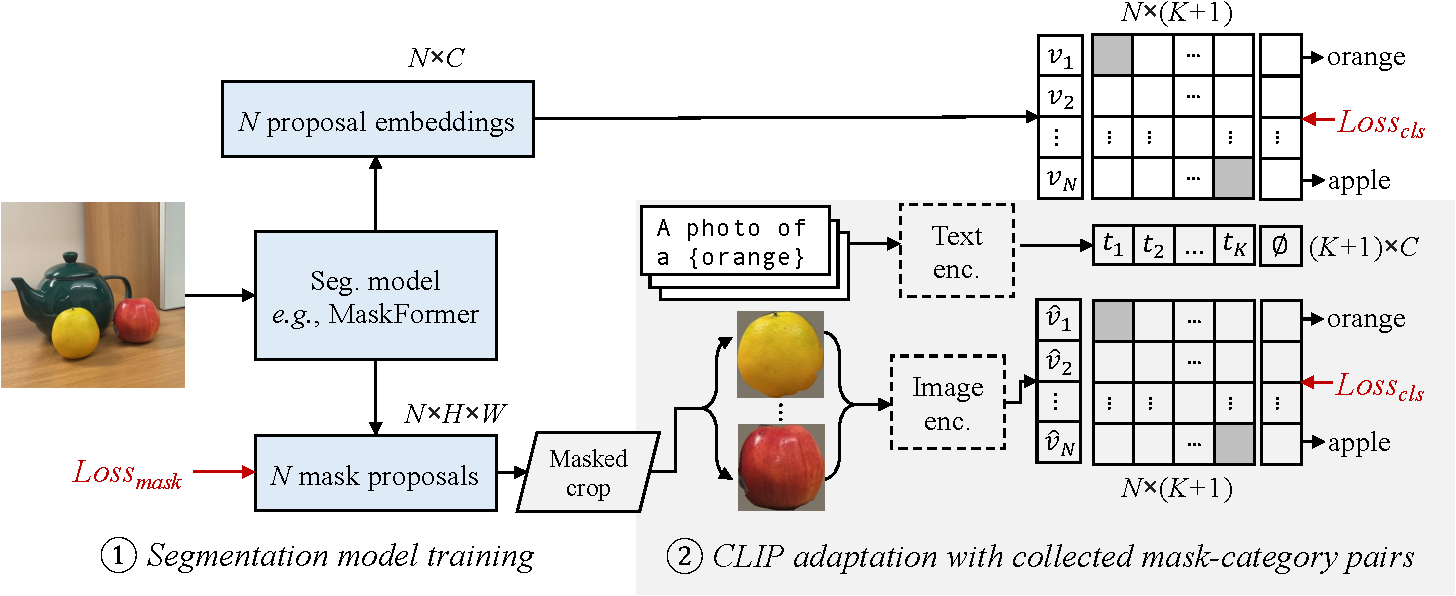
\includegraphics[width=0.98\linewidth]{Fig/fig_CLIP.pdf}
    \caption{OVSeg's oracle analysis of the two-stage open-vocabulary segmentation bottleneck. This placeholder should be replaced by the original Fig.~1 from \emph{Open-Vocabulary Semantic Segmentation with Mask-adapted CLIP}, which contrasts ordinary CLIP classification on masked regions with an oracle classifier and shows why masked-region recognition, not only mask proposal quality, limits two-stage pipelines~\citep{liang2023ovseg}.}
    \label{fig:comparison-ovseg-oracle-placeholder}
\end{figure}

The planned Fig.~\ref{fig:comparison-ovseg-oracle-placeholder} captures the trade-off concisely. OVSeg's oracle analysis shows that even with ground-truth masks, ordinary CLIP classification on masked regions performs poorly on ADE20K-150, while an oracle classifier with imperfect proposals performs much better~\citep{liang2023ovseg}. This result explains why proposal quality alone is not enough. A pipeline needs both accurate spatial support and a region representation that remains compatible with text embeddings. SAN, Mask-Adapter, USE, and ReME all address this interface between masks and text-aligned semantics, but they do so with different assumptions about training data, reference sets, and mask embedding extraction~\citep{xu2023san,yliMaskadapterDevilMasks2025,xwangUseUniversalSegment2024,xxuanReMEDataCentricFramework2025}.

SAM-based systems start from the opposite side. They often produce strong masks from prompts, but they do not decide the semantic target by themselves~\citep{kirillov2023sam,ravi2024sam2}. Grounded-SAM composition therefore attaches a detector, grounding model, MLLM, or agent before SAM. This improves spatial precision, but the semantic decision is only as good as the module that generated the prompt. If Grounding DINO localizes the wrong noun, if an MLLM ignores a relational modifier, or if a video agent chooses the wrong key frame, SAM can still return a visually precise but semantically wrong mask~\citep{liu2024groundingdino,zhouThinkYouSegment2026,huangUnleashingTemporalspatialReasoning2025}.

The practical conclusion is that semantic and spatial errors should be separated whenever possible. For category-level open-vocabulary segmentation, reports should distinguish class recognition, mask proposal quality, and final fusion. For referring and grounded segmentation, reports should distinguish target selection from boundary accuracy. For reasoning segmentation, reports should distinguish target inference, rationale correctness, spatial prompt quality, and final mask overlap. Otherwise, a single number hides whether the failure came from language, semantics, localization, or mask decoding.

\subsection{Training-based adaptation versus training-free composition}

Training-based adaptation and training-free composition solve different deployment problems. Training-based methods, such as OVSeg, SAN, Mask-Adapter, PixelLM, LISA, LENS, MedReasoner, and Affordance-R1, modify parameters or optimize policies so that the model better fits a target interface~\citep{liang2023ovseg,xu2023san,yliMaskadapterDevilMasks2025,renPixellmPixelReasoning2024,xlaiLisaReasoningSegmentation2024,zhuLensLearningSegment2026,yanMedreasonerReinforcementLearning2026,wangAffordancer1ReinforcementLearning2026}. Their advantage is task alignment: they can learn masked-region classification, segmentation tokens, pixel decoders, reward-shaped reasoning, or domain-specific grounding. Their risk is narrowing the original open-vocabulary ability or overfitting to a benchmark's phrasing, label names, or data distribution.

Training-free systems preserve the pretrained models and avoid pixel-label training, but they are not automatically cheap or reproducible. Trident is training-free, yet its result depends on CLIP, DINO, SAM, feature splicing, correlation aggregation, and SAM refinement prompts~\citep{shiyHarnessingVisionFoundation2025}. CLIPer avoids target training, but its fine-grained compensation relies on Stable Diffusion attention maps~\citep{lsunCliperHierarchicallyImproving2025}. ReME uses a refined segment-text reference set, and Grounded-SAM agents may call detectors, MLLMs, LLMs, SAM2, and trackers~\citep{xxuanReMEDataCentricFramework2025,luoConnectingDotsTrainingFree2026}. Thus, ``training-free'' should be reported together with foundation modules, inference time, memory, prompt budget, reference data, and external-tool calls.

RL and preference optimization form a third route. They are training-based, but the target is not ordinary supervised imitation. POPEN, LENS, RISE, SAM-R1, VideoSeg-R1, MedReasoner, and Affordance-R1 optimize response format, localization, mask quality, modality use, or affordance recognition with reward or preference signals~\citep{zhuPopenPreferencebasedOptimization2025,zhuLensLearningSegment2026,zhouReasoningImplicitSelfsupervised2026,huangSamr1LeveragingSam2026,xuVideosegr1ReasoningVideo2026,yanMedreasonerReinforcementLearning2026,wangAffordancer1ReinforcementLearning2026}. This route is promising because segmentation with language is a multi-objective problem. However, reward design can introduce its own bias. A model may learn to satisfy an IoU reward while producing an unfaithful rationale, or satisfy a format reward while providing shallow reasoning. Reward-based papers should therefore report not only final mask scores, but also reward components, rejection behavior, and faithfulness checks.

\subsection{Reasoning capability versus grounding faithfulness}

Reasoning segmentation should not be treated as simply longer referring expression segmentation. The defining question is whether the model can infer the intended target before producing the mask. LISA demonstrates that a \texttt{<SEG>} token can turn an MLLM hidden state into a mask, and that a small amount of ReasonSeg fine-tuning improves implicit-query performance~\citep{xlaiLisaReasoningSegmentation2024}. PixelLM shows that a codebook-based pixel decoder can support multi-target reasoning with lower dependence on external segmentation modules~\citep{renPixellmPixelReasoning2024}. LENS and RISE further show that reasoning and segmentation can be optimized with RL, using rewards over format, localization, masks, or semantic alignment~\citep{zhuLensLearningSegment2026,zhouReasoningImplicitSelfsupervised2026}.

The open problem is faithfulness. A reasoning trace can be plausible even when it did not causally determine the mask. A mask can have high overlap even when the explanation selects the wrong evidence. A grounded response can mention the right object but attach the mask to the wrong region. False-premise work, GSVA's rejection token, grounded visual chat, GLaMM, GroundingSuite, and VBackChecker all point to the same issue: reasoning segmentation must be able to answer, ground, segment, or reject, and the text-mask relation must be checked explicitly~\citep{wuSeeSaySegment2024,xiaGsvaGeneralizedSegmentation2024,zhangLlavagroundingGroundedVisual2024,rasheedGlammPixelGrounding2024,huGroundingSuiteMeasuringComplex2025,guoSeeingBelievingRichContext2026}.

This distinction is even more important in extended domains. In video, the model may answer the query correctly but propagate the mask along the wrong track. In remote sensing, it may choose the right semantic class but fail under scale or rotation. In medicine, it may segment an anatomically plausible region for the wrong clinical reason. In affordance grounding, it may segment the object instead of the functional part used for the action~\citep{zhengVillaVideoReasoning2025,libExploringEfficientOpenvocabulary2026,yanMedreasonerReinforcementLearning2026,wangAffordancer1ReinforcementLearning2026}. Therefore, future comparison protocols should include at least three layers: language or reasoning correctness, grounding or target-selection correctness, and final mask quality.

\subsection{Benchmark and reproducibility gaps}

The first benchmark gap is vocabulary construction. Open-vocabulary segmentation depends on class names, synonyms, descriptions, prompt templates, and label granularity. RENOVATE and FLOSS-style analyses show that improving the textual side of the benchmark can change measured performance, which means that reported gains may reflect better name alignment as well as better visual segmentation~\citep{hhuangRenovatingNamesOpenvocabulary2024,ybenigmimFlossFreeLunch2025}. Papers should therefore publish the exact vocabulary, prompt templates, synonym lists, and any name renovation used at evaluation time.

The second gap is hidden supervision and foundation-model heterogeneity. Methods may use COCO-Stuff, COCO Captions, SA-1B, SAM/SAM2, CLIP, OpenCLIP, DINO, Stable Diffusion, Grounding DINO, MLLM instruction data, generated QA pairs, retrieval reference sets, or target-domain images~\citep{liang2023ovseg,kirillov2023sam,ravi2024sam2,liu2024groundingdino,xxuanReMEDataCentricFramework2025}. Without listing these sources, a comparison can confuse algorithmic improvement with stronger pretraining, larger reference data, or more favorable target-domain exposure.

The third gap is metric fragmentation. Semantic mIoU, mask AP, PQ, cIoU, gIoU, Acc@IoU, $\mathcal{J}\&\mathcal{F}$, rejection accuracy, grounded response metrics, hallucination detection, latency, and TFLOPs answer different questions. Tables~\ref{tab:representative-comparison-evidence} and~\ref{tab:extended-comparison-evidence} show that even representative methods in the same survey report different metrics because they solve different tasks. A mature benchmark suite should not force all tasks into one score, but it should require a minimal reporting checklist: input interface, prompt source, foundation backbones, training data, target-domain usage, output format, metrics, compute, and failure categories.

In summary, the field has moved from asking whether a model can segment unseen category names to asking whether it can ground, reason, verify, and act over masks. This progress is real, but it also makes comparison easier to misuse. The most reliable reading of a result is conditional: a score is meaningful only with its vocabulary, prompts, mask generator, reasoning interface, training data, domain, and metric. Section~\ref{sec:future-directions} therefore turns these comparison gaps into future research directions on standardized protocols, faithful reasoning, efficient composition, and domain-robust evaluation.
